\documentclass[12pt,a4paper,fleqn]{article}

\usepackage[utf8]{inputenc}
\usepackage[T1]{fontenc}
\usepackage[brazil]{babel}
\usepackage{mathptmx}
\usepackage[a4paper,left=2.5cm,right=2.5cm,top=2.5cm,bottom=2.5cm]{geometry}
\usepackage[final]{graphicx}
\usepackage{amsmath,amssymb}
\usepackage{array}
\usepackage{booktabs}
\usepackage{caption}
\usepackage{fancyhdr}
\usepackage{indentfirst}
\usepackage{microtype}
\usepackage[round,authoryear]{natbib}
\usepackage{tikz}
\usepackage{titlesec}
\usepackage[hidelinks]{hyperref}
\usetikzlibrary{arrows.meta,positioning}

\emergencystretch=2em
\setlength{\parindent}{0.75cm}
\setlength{\parskip}{0pt}
\setlength{\mathindent}{1cm}
\linespread{1.0}
\setlength{\headheight}{25pt}
\setlength{\headsep}{12pt}
\setlength{\footskip}{25pt}

\pagestyle{fancy}
\fancyhf{}
\fancyhead[L]{\fontsize{8.5}{9.5}\selectfont\itshape III MCSM\\13--15 de agosto de 2026}
\fancyfoot[C]{\fontsize{8}{9}\selectfont\itshape Anais do III MCSM -- Modelagem Computacional do Sertão Mineiro - 2026}
\renewcommand{\headrulewidth}{0pt}
\renewcommand{\footrulewidth}{0pt}

\titleformat{\section}
  {\normalfont\bfseries}
  {\thesection.}{0.75cm}{\MakeUppercase}
\titlespacing*{\section}{0pt}{12pt}{12pt}
\titleformat{\subsection}
  {\normalfont\bfseries}
  {\thesubsection}{0.75cm}{}
\titlespacing*{\subsection}{0pt}{12pt}{12pt}

\captionsetup{
  font=normalfont,
  labelfont=normalfont,
  labelsep=colon,
  justification=centering,
  singlelinecheck=true,
  skip=6pt
}
\renewcommand{\refname}{REFERÊNCIAS}
\setlength{\bibsep}{0pt}
\setlength{\bibhang}{0.75cm}
\bibpunct{(}{)}{;}{a}{,}{,}
\urlstyle{same}
\newcounter{algoritmo}
\newcommand{\autor}[2]{\noindent\textbf{#1}$^{1}$ - #2\par}
\newcommand{\tituloartigo}{Avaliação do DeepNPTS e de Modelos de Referência para Previsão Mensal de Irradiância Global Horizontal em Localidades de Fábricas de Veículos Elétricos}
% Marcadores longos não alargam as tabelas no rascunho. Depois que um
% marcador é substituído por um número, o próprio número passa a ser exibido.
\newcommand{\resultado}[1]{%
  \ifnum\pdfmatch{^@@}{\detokenize{#1}}>0 --\else #1\fi}

\hypersetup{
  pdftitle={\tituloartigo},
  pdfauthor={Gustavo de Melo Nascimento; Thales Wulfert Cabral; Gustavo Fraidenraich},
  pdfkeywords={Irradiância solar, GHI, previsão probabilística, séries temporais, DeepNPTS}
}

\begin{document}

\begin{center}
  
\includegraphics[width=\textwidth]{banner_iii_mcsm.png}
\end{center}

\vspace{6pt}

\begin{center}
\begin{minipage}{0.98\textwidth}
\centering\bfseries
\MakeUppercase{\tituloartigo}
\end{minipage}
\end{center}

\vspace{12pt}

\autor{Gustavo de Melo Nascimento}{g239679@dac.unicamp.br}
\autor{Thales Wulfert Cabral}{t264377@dac.unicamp.br}
\autor{Gustavo Fraidenraich}{gfraiden@unicamp.br}
\noindent$^{1}$Faculdade de Engenharia Elétrica e de Computação, Universidade Estadual de Campinas -- Campinas, SP, Brasil

\vspace{24pt}

\noindent\textbf{\textit{Abstract.}} \textit{Este artigo avalia o Deep Non-Parametric Time Series Forecaster (DeepNPTS) na previsão mensal de Irradiância Global Horizontal (GHI), com horizonte de um mês, em dez localidades. Dados da National Solar Radiation Database de 2019--2024 são normalizados e quantizados em 128 níveis com parâmetros pré-teste. O DeepNPTS discreto do GluonTS é comparado a três referências simples e seis modelos aprendidos. O protocolo retrospectivo usa 48 alvos de treinamento, 12 origens de teste por localidade, cinco sementes e parâmetros fixos durante o teste. A \textbf{climatologia} obteve o menor MAE médio, \textbf{12,07 W/m$^2$}; o DeepNPTS obteve \textbf{17,70 W/m$^2$} e ficou em \textbf{9º lugar entre 10 métodos}. Para DeepNPTS e DeepAR também se avaliam CRPS e intervalos preditivos de 90\%. Os resultados restringem-se à janela estudada.}

\vspace{12pt}

\noindent\textbf{\textit{Keywords:}} \textit{Irradiância solar, GHI, previsão probabilística, séries temporais, DeepNPTS}

\vspace{24pt}

\section{Introdução}
\label{sec:introducao}

A disponibilidade do recurso solar condiciona o desempenho de sistemas fotovoltaicos. Nesse contexto, previsões de irradiância contribuem para reduzir a incerteza associada ao planejamento e à operação, embora sua utilidade dependa do horizonte, da resolução temporal e dos dados disponíveis. Em particular, previsões mensais podem apoiar decisões de médio prazo ao sintetizar a variação sazonal do recurso \citep{antonanzas2016,voyant2017}.

Entre as grandezas empregadas para caracterizar essa disponibilidade, a Irradiância Global Horizontal (GHI) reúne a irradiância difusa e a componente direta projetada sobre uma superfície horizontal \citep{duffie2013}. Este trabalho prevê a média mensal da GHI, expressa em W/m$^2$ e calculada sobre as 24 horas do dia; portanto, o alvo não corresponde à energia gerada. Os dados provêm da National Solar Radiation Database (NSRDB), que combina observações de satélite e modelos físicos e, por essa razão, fornece uma referência modelada, e não uma medição em solo \citep{sengupta2018}.

A agregação mensal, contudo, produz apenas doze observações por ano e limita a quantidade de exemplos disponíveis para o treinamento. Essa característica torna especialmente importante comparar modelos flexíveis de aprendizado com referências sazonais simples \citep{voyant2017,voyant2022}.

Três referências que não exigem treinamento estabelecem um patamar inicial de comparação. A \textit{persistência} repete a GHI do mês imediatamente anterior; o \textit{sazonal ingênuo} usa a GHI do mesmo mês do ano anterior; e a \textit{climatologia} usa, para cada localidade, a média histórica daquele mês do calendário, calculada somente com o período de treinamento.

Também são avaliados sete modelos aprendidos. XGBoost e o Perceptron Multicamadas (MLP) recebem atributos organizados em tabela; a Rede Neural Recorrente (RNN), a Long Short-Term Memory (LSTM) e a DilatedRNN processam sequências mensais; DeepAR e DeepNPTS produzem uma distribuição preditiva, isto é, vários valores possíveis acompanhados de suas probabilidades. O DeepAR descreve essa distribuição por uma forma contínua parametrizada \citep{salinas2020}. O DeepNPTS, por sua vez, atribui probabilidades aos valores do contexto observado sem impor essa forma paramétrica \citep{rangapuram2023}.

Diante desse cenário, o objetivo deste trabalho é verificar, sob um mesmo protocolo experimental, se modelos aprendidos superam referências sazonais na previsão da GHI do mês seguinte. A análise enfatiza a variante discreta do DeepNPTS proposta por \citet{rangapuram2023} e disponível no GluonTS \citep{alexandrov2020}. Neste texto, \textit{alvo} é o mês cuja GHI se deseja prever, e \textit{origem de previsão} é o último mês conhecido quando a previsão é produzida. Assim, todos os métodos preveem os mesmos meses a partir do mesmo histórico disponível.

\subsection{Principais contribuições}

As principais contribuições são: (i) a avaliação experimental do DeepNPTS, treinado globalmente, para a previsão mensal de GHI em dez localidades; (ii) sua comparação com referências sazonais e modelos aprendidos de diferentes níveis de complexidade; e (iii) a aplicação de um protocolo auditável, com cinco sementes e métricas pontuais e probabilísticas.

Neste trabalho, \textit{auditável} significa que entradas, cortes temporais, configurações, versões de software e artefatos da execução são registrados para conferência. Cada modelo aprendido é executado com cinco sementes, que controlam etapas pseudoaleatórias como a inicialização dos pesos e a amostragem; a repetição permite observar quanto o resultado depende dessa aleatoriedade. As métricas pontuais comparam um único valor previsto com o observado, enquanto as probabilísticas avaliam a distribuição completa e a incerteza informada pelo modelo.

As fábricas servem exclusivamente como pontos de referência geográfica. Em razão do histórico e da janela de teste disponíveis, não se reivindicam pioneirismo, generalização para outros períodos ou regiões, nem superioridade universal.

\section{Sistema e método experimental}
\label{sec:metodo}

A Figura~\ref{fig:sistema} resume o fluxo experimental. Cada bloco é descrito na mesma ordem.

\begin{figure}[!ht]
\centering
\resizebox{\textwidth}{!}{%
\begin{tikzpicture}[
  bloco/.style={draw,rounded corners=1pt,align=center,minimum height=1.35cm,text width=2.7cm,inner sep=4pt},
  seta/.style={-{Latex[length=2mm]},thick},
  node distance=0.45cm
]
\node[bloco] (a) {GHI diária\\NSRDB};
\node[bloco,right=of a] (b) {Auditoria e\\agregação mensal};
\node[bloco,right=of b] (c) {Normalização, quantização\\e entradas sem futuro};
\node[bloco,right=of c] (d) {Modelos globais\\e referências};
\node[bloco,right=of d] (e) {Teste de um passo,\\métricas e comparação};
\draw[seta] (a)--(b);
\draw[seta] (b)--(c);
\draw[seta] (c)--(d);
\draw[seta] (d)--(e);
\end{tikzpicture}%
}
\caption{Fluxo do sistema para previsão mensal de GHI.}
\label{fig:sistema}
\end{figure}

\noindent\textbf{\textit{Dados e auditoria.}} Antes do treinamento, verificam-se datas, duplicidades, lacunas, valores não finitos, GHI negativa e metadados. As médias diárias preservadas derivam de consultas da NSRDB com intervalo de 60 minutos e são agregadas por mês civil \citep{sengupta2018}.

\noindent\textbf{\textit{Transformação e entradas.}} Em cada localidade, os limites mínimo e máximo do período pré-teste colocam a GHI na escala de 0 a 1. Valores fora desses limites são restringidos ao intervalo e representados por um dos 128 níveis disponíveis; essas operações correspondem, respectivamente, à saturação e à quantização. Nenhum alvo do teste é usado para definir a transformação. Os modelos tabulares recebem os 12 valores mensais anteriores, médias móveis, informações de calendário e a localidade. As redes recorrentes processam a sequência dos 12 meses, enquanto DeepNPTS e DeepAR recebem a série transformada e a identificação da localidade. A quantização é uma escolha deste protocolo, não um requisito do DeepNPTS.

\noindent\textbf{\textit{Ajuste e teste.}} Em cada semente, um único modelo global aprende conjuntamente as dez localidades; não se treina um modelo separado para cada uma. As três referências operam diretamente em W/m$^2$ e não são treinadas. Quando há escolha de complexidade, ela ocorre antes do teste, seguida de um novo ajuste com todo o período pré-teste. A avaliação de 2024 avança mês a mês: para prever janeiro, usa-se o histórico disponível até dezembro de 2023; após observar janeiro, esse valor entra no contexto usado para prever fevereiro, e assim sucessivamente. Os parâmetros dos modelos permanecem fixos durante todo o teste. Portanto, os 12 meses não são previstos conjuntamente. Ao final, as previsões transformadas retornam a W/m$^2$, com piso físico zero e sem teto igual ao máximo do treinamento.

\subsection{DeepNPTS e consolidação}

Em termos simples, o DeepNPTS discreto examina os $C$ valores do contexto recente e aprende quanta probabilidade deve atribuir a cada posição desse histórico. A previsão é obtida sorteando valores do próprio contexto conforme essas probabilidades. Assim, o modelo não precisa escolher previamente uma família contínua, como uma distribuição normal ou Student-$t$.

Formalmente, $\ell$ identifica a localidade, $t$ o último mês observado e $\mathbf z_{\ell,t}$ o contexto com $C$ valores. A rede combina esse contexto, atributos de tempo e um vetor aprendido que representa a localidade, denominado \textit{embedding}, para atribuir probabilidade $p_{\ell,t,j}$ à posição $j$. A função de distribuição preditiva $\widehat F$ de um passo é

\begin{equation}
 \widehat F_{\ell,t+1}(x)=\sum_{j=1}^{C}p_{\ell,t,j}
 \mathbb I(z_{\ell,t-C+j}\le x),\qquad \sum_{j=1}^{C}p_{\ell,t,j}=1.
 \label{eq:deepnpts}
\end{equation}

Na Eq.~\eqref{eq:deepnpts}, $\mathbb I$ vale 1 quando a condição ocorre e 0 caso contrário; $x$ é um valor de comparação. No estimador GluonTS 0.16.2, corrige-se apenas o registro dos \textit{embeddings} no PyTorch; a arquitetura, a distribuição e a função de perda RPS (\textit{Ranked Probability Score}) normalizada permanecem oficiais.

Para consolidar as cinco execuções, calcula-se a média das previsões dos modelos pontuais. DeepNPTS e DeepAR produzem 500 amostras por semente; as 2.500 amostras resultantes para cada origem são reunidas, a mediana fornece a previsão pontual e os quantis formam o intervalo preditivo.

\refstepcounter{algoritmo}\label{alg:sistema}
\noindent\textbf{Algoritmo \thealgoritmo: Treinamento global e avaliação}

\noindent\fbox{\begin{minipage}{0.94\textwidth}
\textbf{Entrada:} séries $\mathcal D$, modelos aprendidos $\mathcal A$, referências $\mathcal R$, sementes $\mathcal S$, contexto $C$, horizonte $h$, corte $c$ e origens $\mathcal O$.\\
\textbf{1:} auditar e agregar cada série.\\
\textbf{2:} ajustar transformações antes de $c$ e construir entradas causais.\\
\textbf{3:} para cada $a\in\mathcal A$ e $s\in\mathcal S$, ajustar um modelo global sem usar o teste; $\mathcal R$ não é treinado.\\
\textbf{4:} em cada $o\in\mathcal O$, prever com $\mathcal A\cup\mathcal R$ e parâmetros fixos.\\
\textbf{5:} consolidar as sementes e selecionar $m^\star=\arg\min_m\overline{\mathrm{MAE}}_m$.\\
\textbf{Saída:} previsões, amostras, intervalos, métricas e $m^\star$.
\end{minipage}}

\section{Configuração e métricas}
\label{sec:configuracao}

O produto GOES Aggregated PSM v4 da NSRDB cobre o período de 2019 a 2024 nas dez localidades analisadas \citep{nlr2026}: BYD Camaçari, BMW San Luis Potosí, Ford Rouge, GM Factory Zero, Hyundai Georgia, Lucid Casa Grande, Rivian Normal e Tesla Fremont, Nevada e Texas. O ano de 2019 fornece os 12 meses de histórico necessários para formar a primeira entrada. Em seguida, os 48 alvos de 2020--2023 compõem o treinamento e os 12 alvos de 2024, o teste, resultando em uma divisão cronológica de 80\%/20\%. Em geral, adota-se um contexto de 12 meses; no DeepAR, suas defasagens adicionais ampliam o passado efetivamente consultado para 23 meses.

A complexidade dos modelos é selecionada antes do teste e, quando há seleção, realiza-se em seguida um novo ajuste com todo o período pré-teste. Como os dados de 2024 já foram examinados durante o desenvolvimento, a avaliação tem caráter retrospectivo e exploratório. As sementes 11, 23, 42, 67 e 89 fixam as operações pseudoaleatórias de cinco repetições independentes de cada modelo aprendido; elas não representam cinco divisões diferentes dos dados. A execução ocorre sem GPU, em Linux 6.8.0-1052-azure, com 2 vCPUs x86\_64 e 7,76 GiB de RAM. O ambiente inclui Python 3.12.1, GluonTS 0.16.2, TensorFlow 2.21, Keras 3.15, PyTorch 2.6, scikit-learn 1.9 e XGBoost 3.2.

\begin{table}[!ht]
\centering
\caption{Hiperparâmetros dos modelos aprendidos.}
\label{tab:hiper}
\renewcommand{\arraystretch}{1.02}
\setlength{\tabcolsep}{3pt}
\begin{tabular}{>{\raggedright\arraybackslash}p{2.2cm}>{\raggedright\arraybackslash}p{12.1cm}}
\toprule
\textbf{Modelo} & \textbf{Configuração} \\
\midrule
XGBoost & Profundidade 3; taxa 0,03; amostragens 0,8; peso mínimo 4; $L_1=0,1$; $L_2=10$; até 1.000 árvores; parada 40. \\
MLP & Camadas 64--32; ReLU; L-BFGS; $\alpha=0,05$; até 2.000 iterações. \\
RNN/LSTM & 16 unidades; estado e covariáveis; densa 16 ReLU; Adam 0,001; MSE; lote 32; até 300 épocas; paciência 30. \\
DilatedRNN & Três camadas de 16; saltos 1--2--4; covariáveis; densa 16 ReLU; Adam 0,001; lote 32; até 300 épocas; paciência 30. \\
DeepNPTS & Discreto; contexto 12; camadas 12--12; \textit{embedding} 5; Adam $10^{-5}$; 100 épocas; 100 lotes/época; lote 32; 500 amostras/semente. \\
DeepAR & Camadas 40--40; Student-$t$; \textit{dropout} 0,1; defasagens 1--12; Adam 0,001; 100 épocas; 50 lotes/época; lote 32; paciência 10; 500 amostras/semente. \\
\bottomrule
\end{tabular}
\end{table}

As métricas pontuais avaliam um único número previsto para cada mês e são aplicadas aos dez métodos. As métricas probabilísticas usam o conjunto de valores possíveis e suas probabilidades; por isso, são aplicadas somente a DeepNPTS e DeepAR.

Para definir as métricas pontuais, sejam $\ell$ a localidade, $m$ o modelo e $i=1,\ldots,n_\ell$ o mês avaliado. Denotam-se por $y_{\ell,i}$ a GHI de referência, $\widehat y_{\ell,i,m}$ a previsão, $e_{\ell,i,m}=y_{\ell,i}-\widehat y_{\ell,i,m}$ o erro e $\bar y_\ell$ a média dos $n_\ell$ alvos. Calculam-se

\begin{equation}
\begin{aligned}
 \mathrm{MAE}_{\ell,m}&=n_\ell^{-1}\sum_i|e_{\ell,i,m}|,&
 \mathrm{MSE}_{\ell,m}&=n_\ell^{-1}\sum_i e_{\ell,i,m}^2,\\
 \mathrm{RMSE}_{\ell,m}&=\sqrt{n_\ell^{-1}\sum_i e_{\ell,i,m}^2},&
 R^2_{\ell,m}&=1-\frac{\sum_i e_{\ell,i,m}^2}{\sum_i(y_{\ell,i}-\bar y_\ell)^2},\\
 \mathrm{nRMSE}_{\ell,m}(\%)&=100\,\mathrm{RMSE}_{\ell,m}/\bar y_\ell.&
\end{aligned}
\label{eq:metricas}
\end{equation}

O MAE é o critério principal por expressar diretamente, em W/m$^2$, a distância média entre previsão e referência. MSE e RMSE atribuem peso maior aos erros grandes, e o RMSE retorna à unidade original \citep{hyndman2006}. O $R^2$ indica quanto da variação dos valores é acompanhada pelo modelo, enquanto o nRMSE apresenta o RMSE como percentual da GHI média.

Para que cada localidade tenha o mesmo peso, primeiro se calcula seu MAE e depois se toma a média dos dez resultados. Esse valor, chamado macro-MAE, é $\overline{\mathrm{MAE}}_m=|\mathcal L|^{-1}\sum_{\ell\in\mathcal L}\mathrm{MAE}_{\ell,m}$, em que $\mathcal L$ representa as dez localidades. Para os modelos repetidos em $S=5$ sementes, a coluna DP usa o desvio-padrão amostral $\sqrt{(S-1)^{-1}\sum_s(\overline{\mathrm{MAE}}_{m,s}-\overline{\mathrm{MAE}}_m)^2}$ e mostra a sensibilidade do desempenho à aleatoriedade.

Também se compara o MAE de cada método com o da climatologia nas mesmas dez localidades. Para cada localidade, calcula-se MAE(modelo) menos MAE(climatologia), de modo que uma diferença positiva favorece a climatologia. O intervalo de confiança de 95\% (IC95\%) é obtido com 20.000 reamostragens \textit{bootstrap} das localidades. O teste bilateral de postos sinalizados de Wilcoxon usa as dez diferenças pareadas, e a correção de Holm ajusta os valores de $p$ das nove comparações simultâneas.

DeepNPTS e DeepAR geram $B$ amostras por previsão. Omitindo $\ell$ e $m$ para simplificar, $x_{i,b}$ e $x_{i,c}$ são as amostras de índices $b,c=1,\ldots,B$. O CRPS empírico é

\begin{equation}
 \mathrm{CRPS}_i=B^{-1}\sum_b|x_{i,b}-y_i|-(2B^2)^{-1}\sum_b\sum_c|x_{i,b}-x_{i,c}|.
 \label{eq:crps}
\end{equation}

Quanto menor o CRPS, melhor a distribuição preditiva combina proximidade do valor observado e concentração das previsões. Se $q_{i;0{,}05}$ e $q_{i;0{,}95}$ são os limites que deixam, respectivamente, 5\% das amostras abaixo e acima do intervalo central, e $\mathbb I$ vale 1 quando a condição é verdadeira e 0 caso contrário, então

\begin{equation}
 \mathrm{PICP}_{90}=\frac{100}{n}\sum_{i=1}^{n}\mathbb I(q_{i;0{,}05}\le y_i\le q_{i;0{,}95}),\qquad
 \mathrm{MPIW}_{90}=\frac{1}{n}\sum_{i=1}^{n}(q_{i;0{,}95}-q_{i;0{,}05}).
 \label{eq:intervalos}
\end{equation}

O PICP$_{90}$ informa a porcentagem de valores observados contida nos intervalos de 90\%; o MPIW$_{90}$ informa a largura média desses intervalos em W/m$^2$. Cobertura próxima de 90\% é desejável, mas deve ser analisada junto com a largura, pois um intervalo muito amplo pode cobrir o valor real sem fornecer uma previsão útil \citep{gneiting2007}.

\section{Resultados e discussão}
\label{sec:resultados}

\subsection{Comparação média}

A Tabela~\ref{tab:medias} ordena os métodos do menor para o maior MAE médio entre localidades. A coluna DP mostra quanto o MAE médio variou entre as cinco sementes. Portanto, ela não representa a diferença de desempenho entre localidades. O traço nessa coluna indica que a referência simples não foi repetida com sementes.

\begin{table}[!ht]
\centering
\caption{Métricas médias entre as dez localidades no teste retrospectivo.}
\label{tab:medias}
\setlength{\tabcolsep}{4.5pt}
\renewcommand{\arraystretch}{1.0}
\begin{tabular}{lrrrrr}
\toprule
\textbf{Modelo} & \textbf{MAE} & \textbf{DP} & \textbf{RMSE} & \textbf{$R^2$} & \textbf{nRMSE} \\
 & \textbf{W/m$^2$} & \textbf{W/m$^2$} & \textbf{W/m$^2$} & & \textbf{\%} \\
\midrule
Climatologia    & \resultado{12,07} & -- & \resultado{15,32} & \resultado{0,931} & \resultado{7,64} \\
LSTM            & \resultado{12,22} & \resultado{0,20} & \resultado{15,06} & \resultado{0,919} & \resultado{7,39} \\
RNN             & \resultado{12,55} & \resultado{0,49} & \resultado{15,59} & \resultado{0,910} & \resultado{7,70} \\
DilatedRNN      & \resultado{13,42} & \resultado{0,83} & \resultado{16,20} & \resultado{0,898} & \resultado{7,93} \\
DeepAR          & \resultado{14,18} & \resultado{0,90} & \resultado{17,94} & \resultado{0,892} & \resultado{8,78} \\
XGBoost         & \resultado{14,57} & \resultado{0,14} & \resultado{17,93} & \resultado{0,892} & \resultado{8,78} \\
MLP             & \resultado{16,06} & \resultado{0,46} & \resultado{19,77} & \resultado{0,875} & \resultado{9,70} \\
Sazonal ingênuo & \resultado{16,94} & -- & \resultado{21,37} & \resultado{0,829} & \resultado{10,38} \\
DeepNPTS        & \resultado{17,70} & \resultado{9,22} & \resultado{22,81} & \resultado{0,847} & \resultado{11,33} \\
Persistência    & \resultado{35,09} & -- & \resultado{42,17} & \resultado{0,576} & \resultado{20,89} \\
\bottomrule
\end{tabular}
\end{table}

A \textbf{climatologia} teve o menor macro-MAE, \textbf{12,07 W/m$^2$}; a persistência teve o maior, \textbf{35,09 W/m$^2$}, diferença de \textbf{23,02 W/m$^2$} (65,60\%). O DeepNPTS obteve \textbf{17,70 W/m$^2$}, ficou em \textbf{9º lugar entre 10 métodos} e superou apenas a persistência. Sua diferença para a climatologia foi \textbf{+5,63 W/m$^2$}, com IC95\% pareado [\textbf{3,76; 7,55}] e $p=\textbf{0,0176}$ no teste de Wilcoxon após correção de Holm. Como o intervalo não inclui zero e o valor de $p$ ajustado é menor que 0,05, o protocolo indica vantagem da climatologia sobre o DeepNPTS nas localidades avaliadas. O DP de \textbf{9,22 W/m$^2$} evidencia forte variabilidade entre sementes. Esses resultados se limitam a quatro ciclos anuais de alvos de treinamento e uma janela de teste.

\subsection{DeepNPTS por localidade}

\begin{table}[!ht]
\centering
\caption{Desempenho pontual do DeepNPTS por localidade.}
\label{tab:local}
\setlength{\tabcolsep}{5pt}
\renewcommand{\arraystretch}{1.0}
\begin{tabular}{lrrrr}
\toprule
\textbf{Localidade} & \textbf{MAE} & \textbf{RMSE} & \textbf{$R^2$} & \textbf{nRMSE} \\
 & \textbf{W/m$^2$} & \textbf{W/m$^2$} & & \textbf{\%} \\
\midrule
BMW San Luis Potosí & \resultado{24,52} & \resultado{29,45} & \resultado{0,571} & \resultado{11,88} \\
BYD Camaçari        & \resultado{15,74} & \resultado{20,74} & \resultado{0,693} & \resultado{8,78} \\
Ford Rouge          & \resultado{17,26} & \resultado{23,35} & \resultado{0,909} & \resultado{14,55} \\
GM Factory Zero     & \resultado{17,52} & \resultado{23,14} & \resultado{0,910} & \resultado{14,44} \\
Hyundai Georgia     & \resultado{16,49} & \resultado{20,56} & \resultado{0,859} & \resultado{10,37} \\
Lucid Casa Grande   & \resultado{10,79} & \resultado{13,94} & \resultado{0,965} & \resultado{5,65} \\
Rivian Normal       & \resultado{25,61} & \resultado{30,73} & \resultado{0,840} & \resultado{17,08} \\
Tesla Fremont       & \resultado{15,57} & \resultado{20,16} & \resultado{0,954} & \resultado{9,14} \\
Tesla Nevada        & \resultado{15,17} & \resultado{21,53} & \resultado{0,947} & \resultado{9,69} \\
Tesla Texas         & \resultado{18,33} & \resultado{24,48} & \resultado{0,820} & \resultado{11,72} \\
\bottomrule
\end{tabular}
\end{table}

O menor MAE do DeepNPTS ocorreu em \textbf{Lucid AMP 1 Casa Grande} (\textbf{10,79 W/m$^2$}) e o maior em \textbf{Rivian Normal} (\textbf{25,61 W/m$^2$}), amplitude de \textbf{14,82 W/m$^2$}. Pelo menor MAE local, a LSTM liderou em quatro localidades, a climatologia em três e RNN, DeepAR e sazonal ingênuo em uma cada; o DeepNPTS, em nenhuma. Essa contagem posterior ao teste é apenas descritiva e não substitui o critério macro.

\subsection{Evolução temporal e incerteza}

\begin{figure}[!ht]
\centering
\begin{minipage}[t]{0.49\textwidth}
\centering
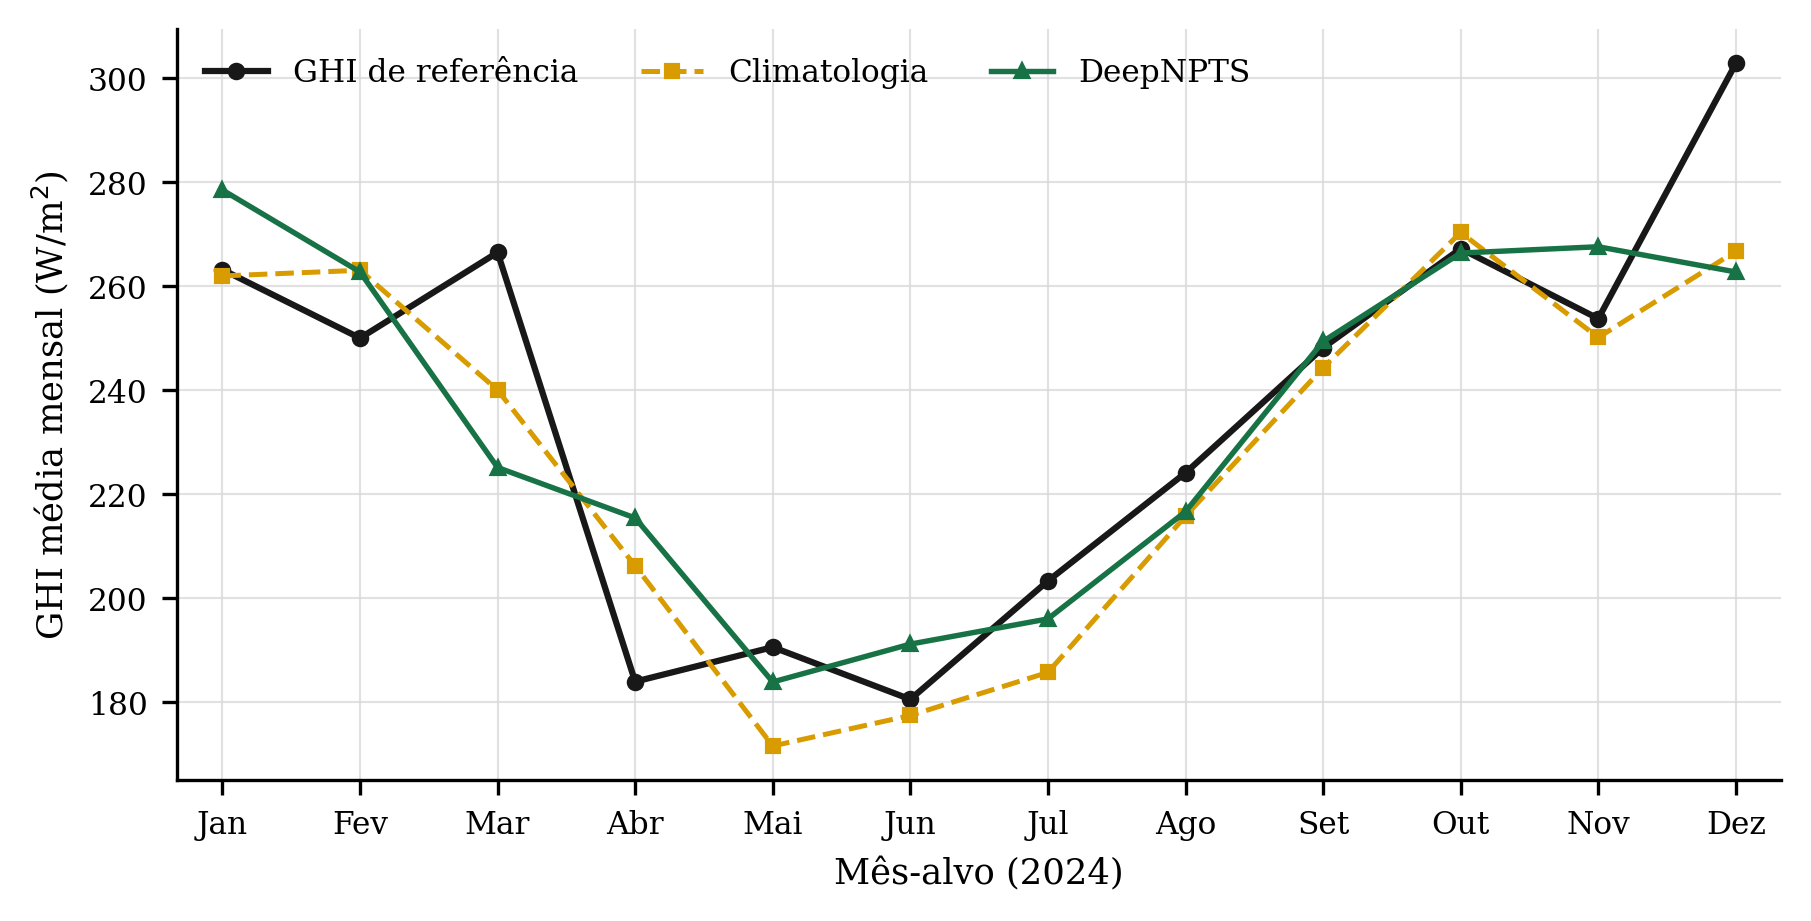
\includegraphics[width=\linewidth]{previsao_mensal_byd_camacari.png}\\
(a) Referência e previsões pontuais.
\end{minipage}\hfill
\begin{minipage}[t]{0.49\textwidth}
\centering
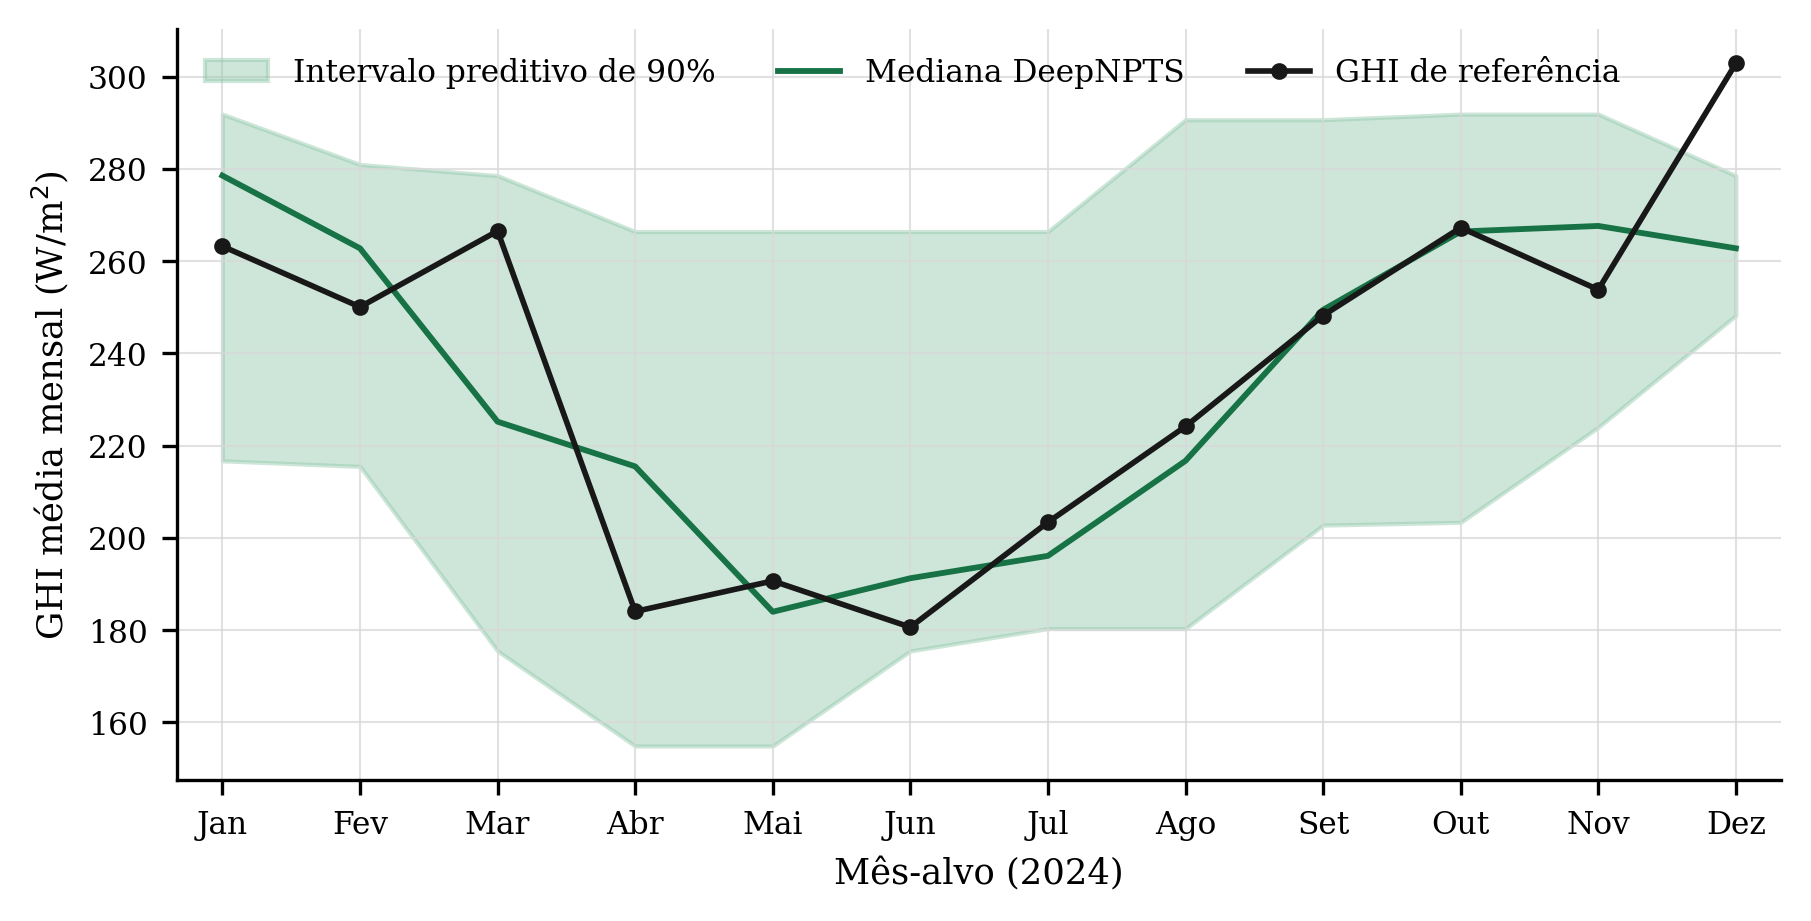
\includegraphics[width=\linewidth]{intervalo_deepnpts_byd_camacari.png}\\
(b) Mediana e intervalo central de 90\%.
\end{minipage}
\caption{GHI de referência modelada e previsões para BYD Camaçari em 2024: (a) DeepNPTS e \textbf{Climatologia}; (b) distribuição preditiva do DeepNPTS.}
\label{fig:byd}
\end{figure}

Em Camaçari, as curvas alternam qual fica mais próxima da referência: o DeepNPTS teve menor erro em 6 dos 12 meses, mas a climatologia apresentou melhor sobreposição no conjunto do ano, com MAE de \textbf{13,14 W/m$^2$}, contra \textbf{15,74 W/m$^2$}.

Na média entre localidades, o DeepNPTS obteve CRPS \textbf{15,90 W/m$^2$}, PICP$_{90}$ \textbf{90,83\%} e MPIW$_{90}$ \textbf{145,56 W/m$^2$}; no DeepAR, foram \textbf{10,83 W/m$^2$}, \textbf{61,67\%} e \textbf{35,50 W/m$^2$}. O intervalo do DeepAR foi mais estreito, mas conteve apenas 61,67\% dos valores observados, abaixo da cobertura nominal de 90\%. O DeepNPTS ficou mais próximo dessa cobertura, porém seus intervalos foram \textbf{4,10 vezes mais largos}. Portanto, a maior cobertura veio acompanhada de menor precisão dos intervalos; além disso, o maior CRPS indica pior desempenho probabilístico global que o DeepAR.

\subsection{Limitações}

A interpretação dos resultados deve considerar quatro ciclos anuais de alvos de treinamento, cinco sementes e uma única janela de teste, já inspecionada durante o desenvolvimento; por isso, a avaliação é retrospectiva. Além disso, a saturação e a quantização afetam os modelos aprendidos, a NSRDB fornece dados modelados, os registros horários brutos não foram preservados e não se utilizaram dados industriais. Assim, qualquer generalização requer avaliação adicional.

\section{Conclusões}
\label{sec:conclusoes}

Este trabalho avaliou o DeepNPTS discreto, treinado globalmente, na previsão mensal de GHI. A \textbf{climatologia} teve o menor macro-MAE (\textbf{12,07 W/m$^2$}). O DeepNPTS obteve \textbf{17,70 W/m$^2$}, ficou em \textbf{9º lugar entre 10 métodos}, superou apenas a persistência e não liderou localidades; seu menor erro ocorreu em Lucid AMP 1 Casa Grande. Frente ao DeepAR, apresentou MAE e CRPS maiores e intervalos 4,10 vezes mais largos, embora com cobertura mais próxima de 90\%.

Os achados não estabelecem superioridade universal. Estudos futuros devem ampliar o histórico, reservar uma janela prospectiva e avaliar outros horizontes, variáveis, saturação e quantização.

\vspace{12pt}
\noindent\textbf{\textit{Agradecimentos.}} Os autores agradecem à FAPEMIG (grant n OET-00243-26).

\begin{thebibliography}{99}

\bibitem[Alexandrov et al.(2020)]{alexandrov2020}
Alexandrov, A. et al. (2020), ``GluonTS: Probabilistic and neural time series modeling in Python'', \textit{Journal of Machine Learning Research}, 21(116), 1--6.

\bibitem[Antonanzas et al.(2016)]{antonanzas2016}
Antonanzas, J. et al. (2016), ``Review of photovoltaic power forecasting'', \textit{Solar Energy}, 136, 78--111.

\bibitem[Duffie e Beckman(2013)]{duffie2013}
Duffie, J.A. e Beckman, W.A. (2013), \textit{Solar Engineering of Thermal Processes}, 4ª ed., cap. 1, Wiley.

\bibitem[Gneiting e Raftery(2007)]{gneiting2007}
Gneiting, T. e Raftery, A.E. (2007), ``Strictly proper scoring rules, prediction, and estimation'', \textit{Journal of the American Statistical Association}, 102(477), 359--378.

\bibitem[Hyndman e Koehler(2006)]{hyndman2006}
Hyndman, R.J. e Koehler, A.B. (2006), ``Another look at measures of forecast accuracy'', \textit{International Journal of Forecasting}, 22(4), 679--688.

\bibitem[National Laboratory of the Rockies(2026)]{nlr2026}
National Laboratory of the Rockies (2026), ``GOES Aggregated: PSM v4 Download API''. Disponível em: \href{https://developer.nlr.gov/docs/solar/nsrdb/nsrdb-GOES-aggregated-v4-0-0-download/}{developer.nlr.gov}; acesso em: 19 jul. 2026.

\bibitem[Rangapuram et al.(2023)]{rangapuram2023}
Rangapuram, S.S. et al. (2023), ``Deep non-parametric time series forecaster'', \textit{arXiv preprint arXiv:2312.14657}.

\bibitem[Salinas et al.(2020)]{salinas2020}
Salinas, D. et al. (2020), ``DeepAR: Probabilistic forecasting with autoregressive recurrent networks'', \textit{International Journal of Forecasting}, 36(3), 1181--1191.

\bibitem[Sengupta et al.(2018)]{sengupta2018}
Sengupta, M. et al. (2018), ``The National Solar Radiation Data Base (NSRDB)'', \textit{Renewable and Sustainable Energy Reviews}, 89, 51--60.

\bibitem[Voyant et al.(2017)]{voyant2017}
Voyant, C. et al. (2017), ``Machine learning methods for solar radiation forecasting: A review'', \textit{Renewable Energy}, 105, 569--582.

\bibitem[Voyant et al.(2022)]{voyant2022}
Voyant, C. et al. (2022), ``Benchmarks for solar radiation time series forecasting'', \textit{Renewable Energy}, 191, 747--762.

\end{thebibliography}

\end{document}
